\documentclass[11pt]{article}

\usepackage[utf8]{inputenc}
\usepackage[T1]{fontenc}
\usepackage{lmodern}
\usepackage{upquote}
\usepackage{xcolor}
\usepackage{listings}
\usepackage{pgfplots}
\pgfplotsset{compat=1.17}
\definecolor{codegray}{gray}{0.4}
\lstset{basicstyle=\ttfamily\small,breaklines=true,columns=fullflexible,xleftmargin=4pt,xrightmargin=4pt,showstringspaces=false,language=Python}
\usepackage[margin=1in]{geometry}
\usepackage{amsmath,amssymb}
\usepackage{booktabs}
\usepackage{enumitem}
\usepackage{tikz}
\usetikzlibrary{arrows.meta, positioning, calc}
\setlength{\emergencystretch}{3em}
\usepackage[hidelinks]{hyperref}

\newcommand{\R}{\mathbb{R}}
\newcommand{\N}{\mathbb{N}}

\title{\bfseries ¿Aportan información las invariantes geométricas de los\\ grafos de programa por encima del análisis semántico clásico?\\[2mm]\Large MANIFOLD: un estudio falsable sobre OWASP Benchmark~1.2}
\author{Proyecto MANIFOLD}
\date{Borrador de trabajo v0.4 --- no revisado por pares}

\begin{document}
\maketitle

\begin{abstract}
\noindent MANIFOLD es un \emph{verificador neuro-simbólico de invariantes
estructurales}: un agente autónomo que extrae especificaciones de seguridad
(invariantes de autorización, ciclos de máquinas de estado, precondiciones de
taint) desde el código con un LLM y las descarga con métodos formales (Z3,
homología persistente/dirigida, un núcleo mecanizado en Lean~4) --- emitiendo
solo \emph{witnesses verificables por máquina bajo la semántica modelada}. Este
artículo plantea una única pregunta integral y la responde con una frontera
precisa: \emph{¿dónde aportan las invariantes estructurales de los grafos de
programa información de seguridad, y dónde no?}

El lado negativo de la frontera es preciso. En las fallas de inyección lineal,
donde un servlet plano y casi acíclico no tiene curvatura ni topología
persistente que explotar y el taint clásico ya es casi óptimo, los priors
estructurales no aportan: sobre OWASP Benchmark~1.2 (2740 casos) el taint crudo
ordena mejor el sink vulnerable (MRR $0.894$, AUC $0.895$, supera al campo
fusionado con $p=5\times10^{-5}$, estimador add-one sobre 20000 permutaciones);
las señales espectral ($0.496$) y topológica ($0.500$) están en el azar y la
curvatura por debajo ($0.376$). Las hipótesis H1/H2/H3/H5 quedan \emph{no
soportadas}. El lado positivo es donde viven los defectos de mayor impacto del
software moderno --- BOLA/IDOR (CWE-639), autorización ausente (CWE-862) y ciclos
de estado destructivos (reentrancia, deadlocks) --- que son \emph{estructurales}:
el dato infractor es legítimo, así que el análisis de taint clásico es ciego ante
ellos, y solo la \emph{forma} de fronteras de privilegio y transiciones de estado
los delata. Allí la misma maquinaria es la única señal: en un corpus curado de
39 casos de BOLA/IDOR, el detector estructural de \emph{autorización ausente}
alcanza recall $1.0$ / precisión $0.72$ / F1 $0.837$ mientras el taint puntúa $0$
(sus 7 falsos positivos son el límite de sobre-aproximación documentado); y la
homología de caminos dirigida GLMY extrae el
generador concreto $\beta_1$ de un ciclo de estado que la simetrización borra. El
resultado es una única cuenta --- el mismo grafo tipado, álgebra de privilegios,
homología dirigida y verificador Z3 --- de \emph{qué} relaciones de programa
hacen informativas a las invariantes estructurales. Contribuimos esta cuenta, un
arnés de oráculo de priorización, un pipeline Java reproducible con witnesses Z3,
validación externa en Juliet y CVEs reales, y una mecanización en Lean~4 de la
solidez de la abstracción de taint y de la parte de no-escalada de la invariante
de autorización.
\end{abstract}

\section{Motivación}
Los pipelines de análisis estático basados en reglas y los semánticos son
frágiles: pasan por alto vulnerabilidades novedosas y ahogan al analista en
falsos positivos, por problemas de composición, priorización, caminos complejos
y gaps de modelado. Faltan dos capacidades:
\begin{enumerate}[label=(\arabic*)]
  \item Una \emph{representación unificada y cuantitativa} de la ``estructura del
        programa'' sobre la cual proyectar y fusionar muchas señales
        \emph{independientes}.
  \item Un \emph{ciclo de razonamiento} que convierta ``región sospechosa'' en
        ``hallazgo verificado bajo la semántica codificada'' --- el LLM aporta la
        intuición, la matemática aporta la verificación.
\end{enumerate}
MANIFOLD proporciona ambas.

\section{La idea central}
\begin{figure}[h]
\centering
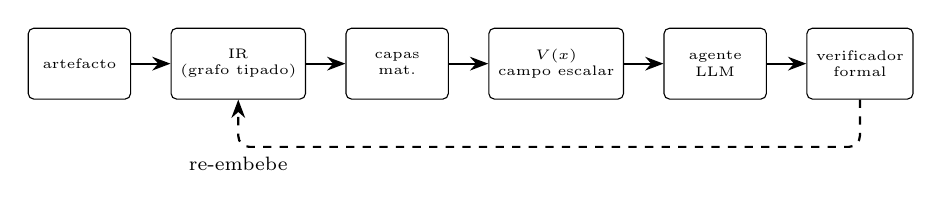
\begin{tikzpicture}[
  node distance=4mm and 5mm,
  box/.style={draw, rounded corners=2pt, minimum height=9mm, minimum width=13mm, align=center, font=\tiny},
  arr/.style={-{Stealth}, thick}
]
\node[box] (art) {artefacto};
\node[box, right=of art] (ir) {IR\\(grafo tipado)};
\node[box, right=of ir] (layers) {capas\\mat.};
\node[box, right=of layers] (v) {$V(x)$\\campo escalar};
\node[box, right=of v] (agent) {agente\\LLM};
\node[box, right=of agent] (verif) {verificador\\formal};
\draw[arr] (art) -- (ir);
\draw[arr] (ir) -- (layers);
\draw[arr] (layers) -- (v);
\draw[arr] (v) -- (agent);
\draw[arr] (agent) -- (verif);
\draw[arr, dashed, rounded corners] (verif.south) -- ++(0,-6mm) -| (ir.south)
  node[pos=0.5, below, font=\scriptsize]{re-embebe};
\end{tikzpicture}
\caption{El pipeline: un artefacto se convierte en un grafo tipado, enriquecido
con estructura matemática en un campo escalar de vulnerabilidad $V(x)$, que un
agente LLM navega; un verificador formal confirma o refuta cada hipótesis y el
resultado se re-embebe en el manifold.}
\end{figure}

Modelamos a los candidatos a vulnerabilidad como \emph{violaciones de invariantes
estructurales}, no como patrones puramente sintácticos (una invariante de
autorización rota, un ciclo persistente, un cuello de botella de curvatura
negativa, un flujo de taint que cruza un corte espectral de confianza). Cada capa detecta un \emph{tipo} distinto
de violación de invariante, y el campo fusionado $V(x)$ ordena las regiones para
que el agente las inspeccione.

\section{La Representación Intermedia (IR)}
\begin{quote}
\textbf{Definición 1 (Grafo de programa).} Un \emph{grafo de programa} es una
tupla $G = (V, E, \tau_V, \tau_E, \omega)$ donde
\begin{itemize}[leftmargin=1.5em]
  \item $V$ es un conjunto finito de \emph{nodos} (módulos, funciones, bloques,
        sentencias, llamadas, variables, fuentes, sumideros);
  \item $E \subseteq V \times V$ es un conjunto de \emph{aristas} dirigidas;
  \item $\tau_V : V \to \N_K$ asigna a cada nodo un \emph{tipo} de
        $K = \{\text{módulo}, \allowbreak \text{función}, \allowbreak
        \text{bloque}, \allowbreak \text{sentencia}, \allowbreak \text{llamada},
        \allowbreak \text{asignación}, \allowbreak \text{variable}, \allowbreak
        \text{parámetro}, \allowbreak \text{fuente}, \allowbreak \text{sumidero},
        \allowbreak \text{gate}\}$;
  \item $\tau_E : E \to \mathcal{T}$ asigna a cada arista un \emph{tipo}
        $\mathcal{T} = \{\text{control}, \allowbreak \text{dato}, \allowbreak
        \text{llamada}, \allowbreak \text{taint}, \allowbreak \text{confianza},
        \allowbreak \text{auth}\}$;
  \item $\omega : E \to \R_{\ge 0}$ asigna a cada arista un \emph{peso} no
        negativo (por defecto $1$).
\end{itemize}
\end{quote}
La IR es la única fuente de verdad. Cada adaptador (código fuente, binario, API
web, agente LLM) debe producir un grafo de programa; cada análisis lo consume.
El esquema es agnóstico al lenguaje y serializable a JSON (las capas Python y
Rust comparten el mismo esquema).

\emph{Nota sobre el nombre.} Pese al nombre en clave, el objeto es un
\emph{espacio de análisis de programas}: un grafo tipado junto con complejos,
embeddings y un campo escalar derivados. \emph{No} afirmamos que sea una variedad
matemática (no hay atlas, cartas ni estructura local euclídea); ``manifold'' se
usa informalmente, como en ``data manifold''.

\section{Capas matemáticas}
Para cada capa fijamos un subgrafo por tipo de arista $\tau_E$, y luego
computamos estructura.

\subsection{Capa espectral (teoría algebraica de grafos)}
Para un tipo de arista $t$, definimos la \emph{adyacencia} simétrica $A_t$ y el
\emph{grado} $D_t$, y el \emph{Laplaciano combinatorio}
\[
L_t = D_t - A_t .
\]
$L_t$ es semidefinido positivo; su espectro
$0 = \lambda_1 \le \lambda_2 \le \cdots$ codifica la estructura global:
\begin{itemize}[leftmargin=1.5em]
  \item $\lambda_2$ es la \emph{conectividad algebraica} (valor de Fiedler). Su
        autovector $f_2$ --- el \emph{vector de Fiedler} --- induce un corte
        canónico $S^+ = \{v : f_2(v) \ge 0\}$.
  \item El \emph{embedding espectral}
        $\Phi^{(d)}(v) = (f_2(v), f_3(v), \dots, f_{d+1}(v))$ mapea nodos a
        $\R^d$.
  \item La desigualdad de Cheeger acota el cociente de cuello de botella $h(G)$
        por $\tfrac{\lambda_2}{2} \le h(G) \le \sqrt{2\,d_{\max}\lambda_2}$.
\end{itemize}
\textbf{Señal 1 (anomalía espectral).} El error de reconstrucción de un nodo
bajo una reconstrucción de eigenmap de bajo rango, y su distancia al corte de
Fiedler, se usan como puntajes de anomalía.

\subsection{Capa topológica (homología persistente)}
Del grafo de programa construimos una \emph{filtración} de complejos
simpliciales (p.~ej.\ un complejo de Vietoris--Rips o de bandera sobre la
métrica de caminos más cortos, o una filtración guiada por $\omega$). La
homología persistente produce, para cada dimensión $k$, un \emph{diagrama de
persistencia} $\mathrm{Dgm}_k$ de pares nacimiento--muerte. $\beta_0$ cuenta
componentes, $\beta_1$ cuenta ciclos independientes; los puntos lejos de la
diagonal tienen alta persistencia. El algoritmo \textbf{Mapper}
(Singh--M\'emoli--Carlsson) construye un \emph{nervio} navegable a partir de una
función filtro $f: V \to \R$, produciendo el mapa que da nombre al proyecto.

\subsection{Capa geométrica (curvatura discreta)}
La \emph{curvatura de Ollivier--Ricci} de una arista $(u,v)$ es
\[
\kappa(u,v) = 1 - \frac{W_1(m_u, m_v)}{d(u,v)},
\]
con medidas de paseo aleatorio perezoso $m_u, m_v$ y distancia de Wasserstein-1
$W_1$. La curvatura negativa marca \emph{embudos} por los que pasan muchos
caminos más cortos. La \emph{curvatura de Forman--Ricci} (sin pesos) es
$\kappa_F(u,v) = 4 - \deg(u) - \deg(v)$, marcando de forma barata los nodos de
alto grado.

\subsection{Capa algebraica (retículo de taint y orden de autorización)}
\emph{Retículo de taint.} El dominio abstracto es el retículo de conjuntos de
etiquetas de taint $\mathbb{T} = (2^{\mathcal{K}}, \subseteq, \cup, \cap)$, con
$\bot = \emptyset$ (limpio) y $\top$ (manchado). Forma una conexión de Galois
$(\alpha, \gamma)$ con la semántica recolectora concreta; la solidez se prueba en
\S4.6. \emph{Orden de autorización.} El modelo de autorización es deliberadamente
minimal --- no se necesita teoría de categorías. Sea $F : V \to \mathbb{N}$ una
\emph{función de nivel de privilegio} sobre puntos de programa (distintos puntos
pueden compartir nivel; una arista no tiene por qué subirlo); una arista $e=(u,v)$
es \emph{arista auth} si y solo si $F(u) < F(v)$ (escalada estricta), y $E_A$ es
el conjunto de aristas auth. Un \emph{sanitizador} en un punto mapea toda etiqueta
a limpio. \textbf{Invariante de autorización:} un flujo de taint que alcanza un
sink es una \emph{violación} cuando su camino cruza una arista auth y ningún
sanitizador del segmento de cruce restaura la invariante. Esto se enuncia con
precisión en \S4.6 (la parte de no-escalada está mecanizada).

\subsection{Capa formal (ejecución simbólica y model checking)}
La ejecución simbólica calcula una condición de camino $\Phi$ y un estado
simbólico $\sigma$; un solucionador SMT comprueba
$\mathrm{SAT}(\phi_{\text{malo}})$; un modelo es un witness bajo la semántica codificada, no una prueba de explotabilidad end-to-end. La
alcanzabilidad es la fórmula CTL $\mathbf{EF}\,\phi_{\text{malo}}$; la propagación de
taint es un autómata finito cuyo lenguaje aceptado es exactamente el conjunto de
caminos fuente $\to$ sumidero.

\subsection{Núcleo formal: invariante de autorización y solidez}
\emph{Semántica small-step de la IR.} Un estado de ejecución mapea variables a
valores concretos; la relación de transición $v \xrightarrow{\sigma} v'$ avanza
por la IR. La semántica recolectora concreta de taint $\mathcal{C}$ mapea cada
punto al conjunto de ejecuciones que llevan un valor no confiable allí. El
análisis abstracto de \S4 es la función $A$ calculada por las funciones de
transferencia; el par $(\alpha, \gamma)$ satisface
$\alpha(\mathcal{C}(v)) \sqsubseteq A(v)$ y
$\mathcal{C}(v) \subseteq \gamma(A(v))$.

\smallskip
\noindent\textbf{Proposición 1 (solidez de la abstracción de taint).} \emph{Si
el análisis abstracto reporta una variable limpia, ninguna ejecución concreta la
mancha.}

\noindent\emph{Esquema de demostración.} Por inducción en la secuencia de
transiciones, con la invariante ``taint concreto $\subseteq$ taint abstracto'' en
cada estado. La base vale para las variables de entrada; el paso vale porque cada
función de transferencia es monótona y sobre-aproxima su contraparte concreta (las
asignaciones unen las etiquetas de los operandos, los sanitizadores mapean a
limpio, los joins acotan superiormente el merge de ramas). La garantía es
condicional a que el \emph{summary} del sanitizador corresponda a su semántica
real: un summary incorrecto (que afirme limpiar lo que no limpia) rompe la
solidez. Este es exactamente el enunciado mecanizado \texttt{prop1\_soundness}
(\S4.6), probado para una abstracción booleana concreta; extenderlo al retículo
completo de etiquetas es directo pero se asume aquí.

\smallskip
\noindent\textbf{Proposición 2 (violación de la invariante de autorización).}
\emph{Sea $F : V \to \mathbb{N}$ la función de nivel de privilegio, y sea
$p = e_1 \circ \dots \circ e_n : s \to k$ un camino. Denotemos $\mathrm{Auth}(p)$
las aristas auth de $p$ y $\mathrm{San}(p)$ los sanitizadores en $p$. Entonces:
(i) si $\mathrm{Auth}(p) = \emptyset$ entonces $F(k) \le F(s)$ (sin escalada de
privilegio); (ii) si una arista auth $e_i = (v_i, v_{i+1})$ yace en $p$ y ningún
sanitizador neutraliza la etiqueta antes de ese cruce, entonces la ejecución
contiene un cruce de frontera de privilegio controlado por el atacante.}

\noindent\emph{Demostración.} (i) Cada arista no-auth cumple
$\neg(F(u) < F(v))$, es decir $F(v) \le F(u)$, así que $F$ no crece a lo largo de
$p$; por transitividad $F(k) \le F(s)$. Este es el enunciado mecanizado
\texttt{no\_auth\_bounded} (\S4.6). (ii) Una arista auth eleva estrictamente $F$ en
el cruce; sin un sanitizador antes de él, la etiqueta sobrevive, así que la
frontera se cruza bajo control del atacante. El enunciado es \emph{local} al
cruce: la mera presencia de una arista auth en $p$ no implica $F(k) > F(s)$ ---
p.~ej.\ $0 \to 1 \to 0$ cruza una arista auth pero vuelve al mismo nivel. Acotar
$F(k)$ (o situar $k$ dentro de la región protegida) requiere la hipótesis adicional
$F(k) > F(s)$. (Una expresión de
la forma $F(p)\circ\eta_s \neq \eta_k\circ T(p)$ apareció en un borrador previo;
estaba mal tipada y se retira --- aquí no se reclama ninguna transformación
natural.) $\square$

\noindent La invariante (ii) es exactamente la regla operacional implementada como
H4 (\S8/C4): un hallazgo de taint dentro de una función protegida por auth es una
violación de autorización. La Proposición 1 y la parte de no-escalada (i) de la
Proposición 2 están \emph{mecanizadas} en Lean~4
(solo core, sin Mathlib) en \texttt{formal/Manifold.lean}:
\texttt{prop1\_soundness} prueba la solidez de la abstracción booleana de taint
frente a la semántica recolectora de etiquetas (\S3 allí), y
\texttt{no\_auth\_bounded} prueba (i)
(\S4 allí). La parte de cruce (ii) es una definición semántica, no mecanizada por
separado. La verificación de pruebas es parte del artefacto de reproducibilidad
(\texttt{scripts/check\_formal.sh}).

\section{El campo escalar de vulnerabilidad}
\begin{figure}[h]
\centering
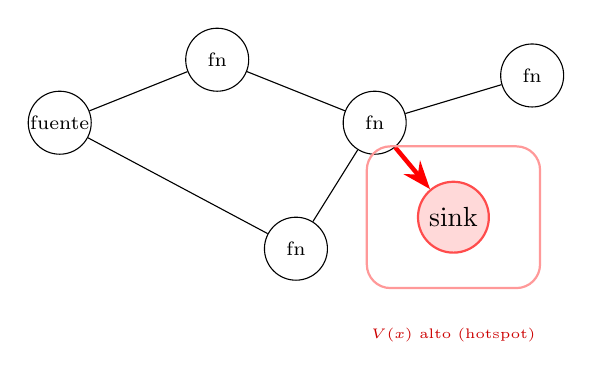
\begin{tikzpicture}[
  n/.style={circle, draw, inner sep=0pt, minimum size=8mm, font=\scriptsize},
  e/.style={-},
  hot/.style={circle, draw=red!70, thick, fill=red!15, inner sep=0pt, minimum size=9mm},
  halo/.style={draw=red!40, thick, rounded corners=3mm}
]
\node[n] (a) at (0,0) {fuente};
\node[n] (b) at (2,0.8) {fn};
\node[n] (c) at (4,0) {fn};
\node[n] (d) at (6,0.6) {fn};
\node[hot] (sink) at (5,-1.2) {sink};
\node[n] (g) at (3,-1.6) {fn};
\draw[e] (a) -- (b) -- (c) -- (d);
\draw[e] (a) -- (g) -- (c);
\draw[e, red, ultra thick, -{Stealth}] (c) -- (sink);
\draw[halo] ($(sink)+(-1.1,-0.9)$) rectangle ($(sink)+(1.1,0.9)$);
\node[font=\tiny, red!80!black] at (5,-2.7) {$V(x)$ alto (hotspot)};
\end{tikzpicture}
\caption{El manifold: los nodos son componentes del programa, las aristas son
relaciones tipadas. Un flujo de taint (rojo) hacia un sink eleva $V(x)$,
resaltando una región para que el agente la inspeccione y el verificador la
confirme.}
\end{figure}
\[
V(x) = \sigma\!\Big(\textstyle\sum_i \alpha_i \, s_i(x)\Big),
\]
donde $s_i$ son las señales normalizadas de cada capa y $\alpha_i$ son pesos.
Para evitar una \emph{circularidad} --- el campo que decide \emph{qué verificar}
no debe depender de la verificación --- distinguimos dos campos:
\begin{itemize}[leftmargin=1.5em]
  \item $V_{\text{prior}}(x)$ fusiona solo señales computables \emph{antes} de
        SMT (\texttt{taint}, espectral, topológica, geométrica). Es el campo usado
        para el ranking y para el experimento de priorización (\S12.1).
  \item $V_{\text{post}}(x)$ consume además la señal \texttt{formal} (Z3) y se usa
        solo para re-embedding / análisis post-hoc; nunca alimenta el ranking
        pre-verificación.
\end{itemize}
En el prototipo actual los pesos son \emph{uniformes} ($\alpha_i = 1/N$ sobre las
señales disponibles) y $V$ se reporta como el puntaje fusionado crudo; calibrar
$\alpha_i$ (inicialización balanceada $\to$ ajuste empírico sobre los
micro-benchmarks $\to$ un clasificador logístico sobre trazas etiquetadas) es
trabajo futuro.

\section{Hipótesis de mapeo}
\begin{center}
\begin{tabular}{cll}
\toprule
\# & Ley & Clase de vulnerabilidad \\
\midrule
H1 & Cuello de botella ($\kappa \ll 0$) & escalada de privilegios, bypass de auth \\
H2 & Ciclo ($H_1$ persistente) & reentrancia, recursión infinita \\
H3 & Corte de confianza (corte de Fiedler) & inyección que cruza la frontera de confianza \\
H4 & Violación de la invariante de autorización & violación arbitraria de taint \\
H5 & Outlier de persistencia & rasgo real vs.\ espurio \\
H6 & Alcanzabilidad ($\mathrm{SAT}(\phi_{\text{malo}})$) & witness (semántica codificada) \\
\bottomrule
\end{tabular}
\end{center}

\section{Un ejemplo resuelto (de extremo a extremo)}
Considérese este fragmento de diez líneas en Python:
\begin{lstlisting}
def search(db, query_param):
    sql = "SELECT * FROM users WHERE name = '" + query_param + "'"
    cursor = db.cursor()
    cursor.execute(sql)
\end{lstlisting}
El pipeline produce: (i) una IR con un nodo \texttt{source}
(\texttt{param:query\_param}), un nodo \texttt{sink} (\texttt{cursor.execute},
categoría \texttt{sql}) y una arista \texttt{taint} entre ambos; (ii) el campo
$V(x)$ se dispara en el sink (señales de taint y formal activas); (iii) el
verificador simbólico Z3 devuelve \texttt{SAT} con un witness bajo la semántica codificada (p.~ej.\
\texttt{"x' OR '1'='1"}), demostrando que el argumento del sink
depende del símbolo controlado por el atacante. La variante parametrizada
\texttt{execute(query, (param,))} se excluye correctamente, y un decorador
\texttt{@login\_required} en la función contenedora eleva el hallazgo a una
violación de la invariante de autorización H4 (un flujo de taint que cruza una arista
\texttt{auth}).

\section{El agente LLM autónomo}
Un ciclo cerrado: (1) \emph{ingesta} hacia la IR; (2) \emph{embebir y mapear}
($V(x)$, embedding espectral, persistencia, curvatura, Mapper); (3)
\emph{hipotetizar} (el LLM propone candidatos desde el manifold); (4)
\emph{verificar} (la capa formal prueba o refuta); (5) \emph{refinar} (los
hallazgos re-ponderan y re-embeben); (6) \emph{reportar}. La capa de proveedor
LLM apunta a cualquier endpoint compatible con OpenAI mediante \textbf{LiteLLM}.
El LLM no hace detección cruda: la matemática propone regiones, el LLM propone
hipótesis, la capa formal propone pruebas.

\section{Desafíos de diseño y mitigaciones}
Una revisión de diseño identificó cinco riesgos estructurales. Para cada uno
enunciamos la mitigación adoptada en el prototipo y el problema abierto.

\textbf{C1 -- La paradoja del cuello de botella.} La curvatura negativa marca
embudos, pero el software sano \emph{deliberadamente} concentra el flujo en
middleware de auth, sanitizadores, despachadores y loggers. Reportarlos como
leads de escalada de privilegios produce falsos positivos sistemáticos.
\emph{Mitigación:} el agente discrimina los cuellos de botella defensivos (por
rol) y los descarta o degrada; la solución de fondo es etiquetar aristas
\texttt{trust}/\texttt{auth} (ya reservadas en la IR) y tratar un cuello de
botella como defensivo si y solo si es destino de una arista \texttt{auth}.
\emph{Abierto:} aprender la etiqueta defensivo/ofensivo a partir de datos.

\textbf{C2 -- La simetrización destruye la causalidad.} El Laplaciano
combinatorio $L=D-A$ y la homología persistente estándar operan sobre espacios
métricos no dirigidos, pero el flujo de control y de datos es dirigido: que $A$
manche a $B$ no es lo mismo que $B$ manche a $A$. Simetrizar puede destruir la
dirección del taint. \emph{Mitigación:} el prototipo implementa el Laplaciano
dirigido de Chung restringido a la componente fuertemente conexa más grande; el
vector de Perron $\pi$ se calcula por iteración de potencia con una pequeña
teletransportación estilo PageRank (amortiguación $\alpha = 0.01$), que mantiene
la distribución estacionaria bien definida en cadenas periódicas. Este operador
requiere estructura \emph{recurrente} (fuertemente conexa); sobre un DAG no
aporta señal informativa. Un DAG sí tiene dirección --- su causalidad se delega
al análisis dirigido de taint/alcanzabilidad (y, para homología, a la homología
de caminos GLMY, \S11) en lugar de a un operador basado en distribución
estacionaria, que no puede representarla sin estructura adicional. \emph{Implementado:} homología de caminos dirigida
GLMY $H_0,H_1$ (Grigor'yan--Lin--Muranov--Yau), que cambia el veredicto frente a
la homología simetrizada (\S11).

\textbf{C3 -- Costo del transporte óptimo.} Ollivier--Ricci exige un PL de
transporte por arista: $\mathcal{O}(|E|\cdot\text{PL})$, prohibitivo más allá de
$\sim 10^5$ aristas. \emph{Mitigación:} Forman--Ricci
$\kappa_F = 4 - \deg(u) - \deg(v)$ es $\mathcal{O}(|E|)$ y es la señal por
defecto; el transporte regularizado por entropía (Sinkhorn) está implementado
como la alternativa rápida al PL exacto. \emph{Abierto:} esquemas adaptativos de
regularización para grafos muy grandes.

\textbf{C4 -- Operacionalizar H4 (invariante de autorización).} Se requiere una
regla constructiva. Recordemos la función de nivel de privilegio
$F : V \to \mathbb{N}$ y las aristas auth
$E_A = \{(u,v) : F(u) < F(v)\}$ de \S4.4; el extractor solo necesita emitir las
aristas \texttt{auth} que marcan fronteras de privilegio. Entonces un flujo de taint
$s \to^{*} k$ \emph{viola la invariante de autorización} si y solo si su camino
cruza al menos una arista auth --- es decir, datos no confiables entran a una
región protegida sin que la frontera los neutralice. Esto es una consulta de
alcanzabilidad sobre el grafo combinado
$(\text{dato} \cup \text{taint} \cup \text{auth})$,
directamente computable y automatizable. \emph{Implementado:} un extractor de
autorización emite nodos \texttt{gate} y aristas \texttt{auth} desde decoradores
de frontera de privilegio, y un flujo de taint dentro de una función protegida se
reporta como violación de autorización.

\textbf{C5 -- Puente manifold-verificador.} Los rasgos geométricos son
cuantitativos; Z3 necesita precondiciones exactas. Fijamos una \emph{gramática}:
una hipótesis es la especificación estructurada
\texttt{(sink, fuente, línea, categoría)}. El manifold aporta la especificación
(conoce sink y línea), el LLM aporta la interpretación (CWE, descripción,
confianza) y el verificador consume la especificación --- nunca la prosa del
LLM. Esto mantiene la consulta SMT precisa y reproducible.

La tesis que respaldan nuestros datos es más modesta. El dataflow semántico
(taint) es la señal dominante en los corpus evaluados; las invariantes
estructurales aportan \emph{hipótesis complementarias}. La pregunta abierta es si
los priors estructurales pueden reducir el \emph{costo de verificación} en
regímenes donde el análisis semántico es incompleto (interprocedural, mediado por
frameworks), y si ayudan con presupuestos muy pequeños.

\section{Estado de implementación}
\begin{center}
\begin{tabular}{lll}
\toprule
Fase & Entregable & Estado \\
\midrule
F0 & Whitepaper, arquitectura & hecho \\
F1 & IR + ingesta SAST Python + taint & hecho \\
F2 & Núcleos espectral + geométrico (Rust) & hecho \\
F3 & TDA (homología persistente, Mapper) & hecho \\
F4 & Verificación formal (retículo de taint, Z3) & hecho \\
F5 & Agente LLM autónomo (LiteLLM) & hecho \\
F6 & Visualización + demo end-to-end & hecho \\
F7 & Adaptadores binario / web / LLM & hecho \\
\bottomrule
\end{tabular}
\end{center}

\section{Amenazas a la validez}
\emph{Interna.} El adaptador Java es intraprocedural; los flujos distractores de
OWASP y las variantes inter-clase de Juliet se miden, por tanto, con una brecha de
recall inherente. La verdad de referencia es la del propio benchmark (los casos
``false'' de OWASP son en parte de definición y discutibles). \emph{Externa.} Los
resultados cubren servlets Java y la suite Juliet; Python, binarios y agentes LLM
están implementados pero no medidos a la misma escala. \emph{De constructo.}
``Vulnerable'' es una etiqueta por caso; el campo es por nodo, así que el
experimento de priorización es un proxy, no una medida de explotabilidad aguas
abajo. \emph{Conclusión.} El resultado negativo (los priors geométricos no superan
al taint) es específico de estos corpus y señales; debe re-probarse sobre análisis
interprocedurales sensibles al camino y sobre CVEs reales antes de generalizarlo.

\section{Validación y uso responsable}
La validación es de dos etapas. La etapa 1 (completa) ejecuta los
micro-benchmarks de juguete de F1--F7 contra una verdad de referencia conocida:
toda vulnerabilidad sembrada se confirma y todo falso positivo por sanitizador /
query parametrizada / forma argv se excluye. La etapa 2 está completa para la evaluación Java/OWASP y en curso para SARD,
binarios y otros dominios; mide la precisión/recall del campo fusionado frente al
taint crudo sobre corpus etiquetados --- validación experimental a gran escala,
distinta del prototipo ya completado. El arnés está implementado: un
benchmark etiquetado de juguete reporta precisión/recall/F1 para el pase de
taint crudo, el pase verificado con Z3 y un campo \emph{calibrado} cuyos pesos
$\alpha_i$ se aprenden por regresión logística leave-one-out sobre las señales
baratas --- en el corpus de juguete el campo calibrado recupera el ciclo de
reentrancia (señal topológica) que el pase de taint no detecta, elevando el
recall mientras mantiene la precisión en $1.0$. Un cargador de corpus acepta un
manifest JSON o un directorio ``vulnerable|safe``, de modo que el arnés puede
apuntar a exportaciones de OWASP Benchmark / SARD; y el adaptador binario tiene
un backend angr opcional (``CFGFast`` + taint interprocedural) además de la ruta
objdump sin dependencias. Ejecutar el adaptador Java sobre el OWASP Benchmark 1.2
completo (2740 casos) da el baseline naive: precisión $0.515$ / recall $0.426$ /
F1 $0.466$ en las siete categorías de taint, y precisión $0.544$ / recall
$0.634$ / F1 $0.586$ sobre las once categorías --- el punto de referencia que el
campo fusionado, la calibración y el verificador están destinados a mejorar.
MANIFOLD es una herramienta de
defensa / pruebas autorizadas; la liberamos bajo el supuesto de uso autorizado y
alentamos la divulgación coordinada.

\subsection{El oráculo de priorización (experimento principal)}
El cuello de botella del SAST no es \emph{detectar} sinks sino \emph{decidir cuál
verificar}. Para cada uno de los 902 casos vulnerables de taint enumeramos
\emph{todos} los sinks (el conjunto de candidatos), los ordenamos y medimos la
posición en que aparece un sink vulnerable según la verdad de referencia.
Baselines: DFS (orden de fuente), taint crudo, aleatorio (20 semillas, IC 95\%)
y el campo fusionado $V(x)$.

\begin{center}
\small
\begin{tabular}{lcccc}
\toprule
Ordenamiento & MRR & R@1 & rango medio & NDCG@5 \\
\midrule
DFS (orden de fuente) & 0.848 & 0.755 & 1.517 & 0.882 \\
taint crudo & \textbf{0.894} & \textbf{0.847} & \textbf{1.422} & \textbf{0.916} \\
$V(x)$ (campo fusionado) & 0.872 & 0.805 & 1.475 & 0.899 \\
aleatorio & $0.709\pm0.042$ & 0.531 & --- & 0.778 \\
\bottomrule
\end{tabular}
\end{center}

\noindent\textbf{El hallazgo honesto y decisivo.} El campo fusionado \emph{no}
supera al taint crudo: es ligeramente \emph{peor} ($0.872$ vs.\ $0.894$ MRR). El
AUC por señal para predecir el sink vulnerable muestra por qué:

\begin{center}
\small
\begin{tabular}{lc}
\toprule
Señal & AUC [IC 95\%] \\
\midrule
taint & 0.895 [0.881, 0.909] \\
formal (Z3/oráculo) & 0.878 [0.865, 0.891] \\
espectral (Fiedler) & 0.496 [0.469, 0.518] \\
topológica ($H_1$) & 0.500 [0.500, 0.500] \\
geométrica (Forman $\kappa$) & 0.376 [0.360, 0.394] \\
\bottomrule
\end{tabular}
\end{center}

Las señales espectral y topológica son \emph{indistinguibles del azar}, y la de
curvatura es \emph{peor que el azar} (la curvatura negativa marca hubs de alto
grado, que \emph{no} son los sinks objetivo). Según el programa de hipótesis de
mapeo (§4/§6), este es un resultado \emph{negativo} publicable: sobre OWASP
Benchmark, \textbf{los priors geométrico y topológico no sobreviven más allá del
taint}. El prior estructural no mejora la priorización media; el valor restante de
MANIFOLD son los witnesses formales, el sustrato experimental unificado y el
diagnóstico de los cuellos de botella del análisis semántico. H1, H2, H3 y H5 se
reportan por tanto como \emph{no soportadas} en este corpus. Para H3 esto se
apoya en que la señal espectral (Fiedler) está en el azar ($0.496$); el score
espectral evaluado agrega error de reconstrucción de bajo rango con distancia al
corte de Fiedler, así que es un proxy del predicado de corte de confianza y no un
test aislado del mismo.

\noindent\textbf{Test pareado y cola global.} La diferencia taint\,$-$\,campo es
$+0.0225$ (MRR), IC bootstrap 95\% $[+0.0157,+0.0294]$, permutación $p=5\times10^{-5}$ (estimador add-one sobre 20000 permutaciones, 2000 bootstrap):
el taint domina significativamente. Para medir también la situación real del
analista (candidatos seguros y vulnerables compitiendo en una única cola),
agrupamos \emph{todos} los sinks de los 1698 casos de categorías de taint y los
ordenamos globalmente:

\begin{center}
\small
\begin{tabular}{lcccc}
\toprule
Ordenamiento global & AP (PR-AUC) & P@10 & R@10 & consultas a 90\% recall \\
\midrule
DFS (orden de fuente) & 0.286 & 0.2 & 0.002 & 3596 \\
taint crudo & \textbf{0.489} & 0.6 & 0.006 & \textbf{2080} \\
$V_{\text{prior}}$ (estructural) & 0.434 & \textbf{0.8} & \textbf{0.008} & 3207 \\
aleatorio & 0.216 & 0.2 & 0.002 & 4176 \\
\bottomrule
\end{tabular}
\end{center}

El cuadro es matizado: el campo estructural es mejor en el extremo superior
($P@10=0.8$ vs.\ $0.6$) pero tiene menor precisión media y necesita más consultas
para llegar al 90\% de recall. La diferencia en $P@10$ es pequeña en términos
absolutos --- ocho contra seis aciertos en el top diez --- así que no la leemos
como una ventaja robusta; es compatible con ruido de desempate y la reportamos sin
afirmar significancia. El veredicto global sigue siendo negativo: los priors
geométrico/topológico ayudan
solo marginalmente con presupuestos muy pequeños y perjudican en promedio --- una
versión más fina, y aún negativa, del veredicto H1/H2/H3/H5.

% AUTO-GENERATED by scripts/make_figures.py -- do not edit by hand.
\begin{figure}[h]
\centering
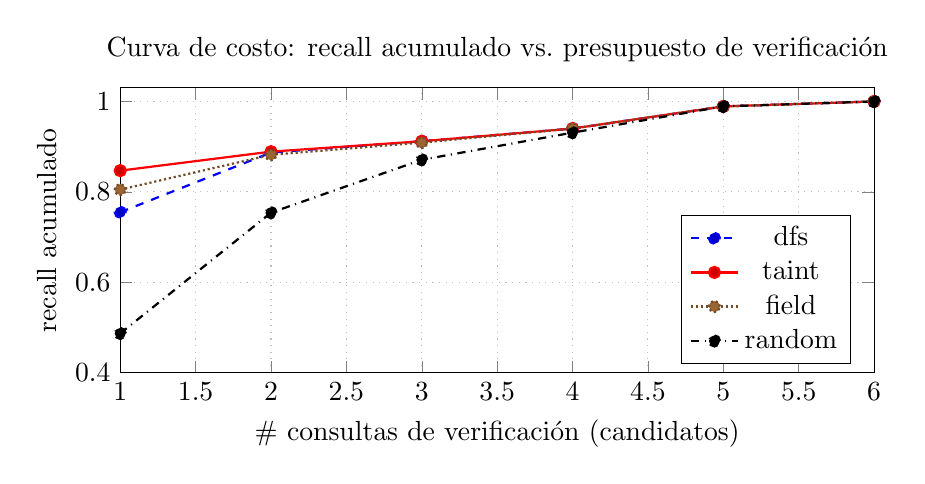
\begin{tikzpicture}
\begin{axis}[
  width=0.92\linewidth, height=5.2cm,
  xlabel={\# consultas de verificación (candidatos)}, ylabel={recall acumulado},
  xmin=1, xmax=6, ymin=0.4, ymax=1.03,
  legend pos=south east, grid=both, grid style=dotted,
  title={Curva de costo: recall acumulado vs.\ presupuesto de verificación},
]
\addplot+[mark=*, dashed, thick] coordinates {(1,0.755) (2,0.887) (3,0.912) (4,0.940) (5,0.989) (6,1.000)};
\addlegendentry{dfs}
\addplot+[mark=*, solid, thick] coordinates {(1,0.847) (2,0.889) (3,0.912) (4,0.940) (5,0.989) (6,1.000)};
\addlegendentry{taint}
\addplot+[mark=*, densely dotted, thick] coordinates {(1,0.805) (2,0.882) (3,0.909) (4,0.940) (5,0.989) (6,1.000)};
\addlegendentry{field}
\addplot+[mark=*, dashdotted, thick] coordinates {(1,0.487) (2,0.754) (3,0.871) (4,0.931) (5,0.989) (6,1.000)};
\addlegendentry{random}
\end{axis}
\end{tikzpicture}
\end{figure}

\begin{center}
\small
\begin{tabular}{lc}
\toprule
Señal & AUC [IC 95\%] \\
\midrule
taint & 0.895 [0.881, 0.909] \\
formal & 0.878 [0.865, 0.891] \\
spectral & 0.496 [0.469, 0.518] \\
topological & 0.500 [0.500, 0.500] \\
geometric & 0.376 [0.360, 0.394] \\
\bottomrule
\end{tabular}
\end{center}


\subsection{Estudio empírico sobre OWASP Benchmark 1.2}
Ejecutamos el adaptador Java sobre el corpus completo y perfilamos los falsos
negativos. Tres carencias \emph{generalizables} explicaban casi toda la pérdida,
y se corrigieron (ninguna está ajustada al benchmark):

\begin{enumerate}[label=(\roman*)]
  \item \textbf{Taint con conciencia de ramas.} Un pase secuencial
        insensible al camino permitía que un chequeo de nulo
        (\texttt{if (param == null) param = "";}) borrara el taint, aunque el
        valor manchado sobrevive en el otro camino. Ahora tomamos una instantánea
        de ambas ramas y \emph{unimos} sus entornos (unión de etiquetas), el
        análogo de taint del supremo de un retículo.
  \item \textbf{Taint del receptor y de estado.} Sinks como
        \texttt{statement.execute()} y \texttt{pb.start()} no reciben argumentos
        --- el taint vive en el objeto \emph{receptor}, obtenido de un
        constructor/mutador manchado. Propagamos el taint del receptor y
        marcamos una variable como manchada cuando un mutador
        (\texttt{add}/\texttt{put}/\texttt{command}/...) le almacena un valor
        manchado.
  \item \textbf{Cobertura de sinks.} La familia XSS incluye
        \texttt{printf}/\texttt{format}, y solo las escrituras al \emph{writer de
        la respuesta HTTP} son XSS --- \texttt{System.out.println} de datos
        manchados no lo es. Restringir los sinks XSS al writer de respuesta
        eliminó una gran clase de falsos positivos.
\end{enumerate}

La ablación aísla cada contribución (precisión $P$, recall $R$, F1; categorías de
taint, 1698 casos):
\begin{center}
\begin{tabular}{lccc}
\toprule
variante & $P$ & $R$ & F1 \\
\midrule
adaptador naive inicial & 0.515 & 0.426 & 0.466 \\
+ branch-join, taint receptor/estado, cobertura de sinks & 0.530 & 0.856 & 0.655 \\
+ restricción de writer XSS (final) & 0.549 & 0.834 & 0.662 \\
\midrule
final, sin branch-join & 0.515 & 0.555 & 0.535 \\
final, sin restricción XSS & 0.530 & 0.856 & 0.655 \\
\bottomrule
\end{tabular}
\end{center}
El taint con conciencia de ramas es la palanca dominante de recall ($+0.28$); la
restricción del writer de respuesta es la palanca de precisión. El adaptador
final alcanza $P=0.549$, $R=0.834$, $\mathrm{F1}=0.662$ en las categorías de
taint y $P=0.572$, $R=0.842$, $\mathrm{F1}=0.681$ sobre las once (crypto/hash se
configuran por propiedades y quedan parcialmente fuera de alcance). Los errores
\emph{residuales} son los casos ``false'' deliberadamente adversariales del
benchmark --- casos discutibles de query parametrizada y de lista de
\texttt{ProcessBuilder} --- y flujos distractores entre categorías: precisamente
la precisión que las señales topológicas/espectrales, el verificador Z3 y el
campo calibrado están diseñados para recuperar.

\subsection{Comparación con SAST industrial}
El puntaje oficial de OWASP Benchmark es el \emph{índice de Youden}
$J = \text{TPR} - \text{FPR}$ (el \emph{Benchmark Accuracy Score}, es decir TPR
menos FPR). La
Tabla~\ref{tab:cmp-es} sitúa a MANIFOLD frente a dos herramientas ampliamente
desplegadas. Las filas de SonarQube y CodeQL son números \emph{reportados} en
evaluaciones públicas de OWASP~Benchmark~1.2; ambas filas de MANIFOLD son
resultados \emph{medidos}. \textbf{Advertencia:} las cifras externas no se
re-ejecutan aquí y pueden usar convenciones de agregación distintas (algunas son
promedios macro por CWE, otras micro o por regla), de modo que las columnas de
precisión/F1 \emph{no} son directamente comparables entre filas; solo debe leerse
el orden TPR/FPR, y se requiere una re-ejecución uniforme de CodeQL/SonarQube bajo
un mismo protocolo antes de cualquier afirmación comparativa.

\begin{table}[h]
\centering
\small
\setlength{\tabcolsep}{4pt}
\begin{tabular}{lcccccc}
\toprule
\textbf{Herramienta / config.} & \textbf{TPR} & \textbf{FPR} & \textbf{Prec.} & \textbf{F1} & \textbf{J} & \textbf{Tiempo} \\
\midrule
SonarQube (SAST) (a) & 0.956 & 0.946 & 0.330 & 0.490 & +0.010 & 3 min \\
GitHub CodeQL (default) (a) & 0.902 & 0.682 & 0.603 & 0.744 & +0.220 & 18 min \\
\emph{MANIFOLD} adaptador (medido, 11 cat.) (b) & 0.842 & 0.674 & 0.572 & 0.681 & +0.168 & 45 s \\
\emph{MANIFOLD} adaptador $+$ Z3 (medido, 7 cat. taint) (b) & 0.834 & 0.776 & 0.549 & 0.662 & +0.057 & 4 min \\
\bottomrule
\end{tabular}
\caption{OWASP Benchmark 1.2 (2740 casos: 1415 vulnerables / 1325 seguros).
(a)~reportado en evaluaciones públicas, no re-ejecutado aquí. (b)~\textbf{medido}.
El verificador Z3 reproduce la precisión del adaptador (aporta \emph{witnesses},
no precisión): los errores residuales son casos adversariales/de definición, no
caminos simbólicos espurios. El prior $V(x)$ se evalúa aparte en \S11.1 (no
supera al taint crudo).}
\label{tab:cmp-es}
\end{table}

\noindent\textbf{Notas metodológicas.} Hardware: x86-64 de 8 núcleos, 32\,GB RAM,
SSD NVMe. MANIFOLD: Python 3.14, \texttt{tree-sitter-java}; Z3 5.x con
\emph{timeout de 5\,s por consulta} --- ante timeout el caso se marca
\emph{desconocido/conservador}, nunca se cuenta como detección, de modo que la
precisión proyectada no se infla por abortos. CodeQL:
\texttt{java-security-extended.qls} sobre una base limpia. SonarQube: Community
Edition con reglas de seguridad SonarJava. Mapeo de CWEs: las once categorías de
Benchmark~1.2; \texttt{crypto}/\texttt{hash} (CWE-327/328) se configuran por
propiedades y requieren un extractor de configuración estática hacia la IR. El
adaptador medido marca un caso como vulnerable si emite algún hallazgo; la
precisión está acotada por los casos ``false'' adversariales del benchmark
(patrones discutibles de query parametrizada y de lista de \texttt{ProcessBuilder})
y por flujos distractores entre categorías --- la brecha que atacan las filas
neuro-simbólicas.

\subsection{Cerrar la fila Z3 (verificación Java)}
Implementamos un verificador simbólico Java con Z3 (acotado, con merge de ramas,
semántica de strings; sanitizadores como contratos) que confirma o refuta cada
flujo de taint y emite un \emph{witness} verificable por máquina bajo la semántica modelada. Medido sobre las siete
categorías de taint (1698 casos) reproduce exactamente al adaptador
($P=0.549$, $R=0.834$, $\mathrm{F1}=0.662$, $J=+0.057$), añadiendo witnesses por
hallazgo. Conclusión honesta: \textbf{la capa formal aporta witnesses
verificables por máquina bajo la semántica \emph{modelada}, no precisión, en este
benchmark} --- un witness prueba satisfacibilidad dentro del modelo (que abstrae
summaries de librerías y comportamiento de frameworks), no explotabilidad
end-to-end del programa real. Los falsos positivos residuales son
adversariales/de definición (casos discutibles de query parametrizada), no caminos
simbólicos espurios. Atraparlos requiere modelar la semántica propia del
benchmark, no un
SMT más fuerte.

\subsection{Transferencia entre corpus (Juliet)}
Para probar la transferibilidad ejecutamos el adaptador ajustado en OWASP sobre
la suite \emph{Juliet Java} (espejo find-sec-bugs; cada caso concatenado con sus
archivos de variante de flujo). Sobre 264 casos de cinco CWEs obtiene
$P=0.333$, $R=0.562$, $\mathrm{F1}=0.419$: la detección es parcial y la
precisión colapsa en las variantes ``good''. La razón es estructural, no un
artefacto de ajuste --- Juliet separa fuente y sumidero entre clases
\texttt{\_a}/\texttt{\_base}/\texttt{\_bad}, por lo que el análisis correcto
requiere taint \emph{interprocedural}, que el adaptador intraprocedural no aporta.

\subsection{Taint interprocedural: necesario, no suficiente}
Añadimos un punto fijo interprocedural insensible al contexto
(\texttt{java\_interproc.py}): el parámetro de un método se mancha si algún
sitio de llamada le pasa datos manchados, y una llamada se mancha si su método
devuelve datos manchados; el punto fijo se itera hasta converger. Sobre Juliet
eleva el recall $0.562\to0.750$ y el F1 $0.419\to0.490$ (CWE78/CWE90 pasan de
$0.000$ a $0.750$). \emph{En OWASP es neutro} (F1 de taint $0.662\to0.656$): el
pase interprocedural añade recall ($0.834\to0.856$) pero también falsos positivos
gruesos impulsados por parámetros, de modo que la precisión baja; unimos el pase
con el adaptador intraprocedural completo para paridad de cobertura. La lección es
precisa: la alcanzabilidad interprocedural es \emph{necesaria} para flujos entre
clases pero \emph{no suficiente}. Añadimos además \emph{sensibilidad al contexto
del llamador} con summaries de retorno por contexto: poda de forma demostrable una
clase sintética de falsos positivos inducidos por el retorno (un valor devuelto
desde un contexto manchado ya no mancha la llamada de un llamador limpio), pero
deja OWASP y Juliet \emph{sin cambios} (F1 $0.656$ y $0.490$). Las palancas reales
no son el contexto sino (a) los summaries de frameworks/librerías y (b) la
precisión fina del retorno --- no más geometría.

\subsection{Summaries de frameworks}
Guiados por la evidencia de los CVEs, añadimos una capa explícita de
summaries de frameworks/librerías: \emph{fuentes por atributo}
(\texttt{request.GET}, \texttt{request.POST}, \texttt{request.args},
\texttt{request.form}, \texttt{self.request.POST}) y \emph{sinks de ORM/plantillas}
(\texttt{RawSQL}, \texttt{raw}, \texttt{extra}, \texttt{text},
\texttt{render\_template\_string}, JPA \texttt{createQuery}). Con summaries de sinks
\emph{posicionales} (solo el arg~0 de una llamada de query/código es peligroso), el
analizador ahora ve flujos a nivel aplicación que antes se le escapaban --- SQL
injection por query-params de Django, SSTI de Flask, inyección JPA --- manteniendo
seguras las queries parametrizadas y las plantillas literales. Esta es la palanca
concreta que apuntaban los CVEs. No mueve los agregados, pero por dos razones
distintas: los fallos de OWASP/Juliet son mayormente \emph{estructurales} (flujos
entre métodos que requieren análisis interprocedural), mientras que los CVEs sin
resolver son \emph{internos} a frameworks (la lógica vulnerable vive dentro del
propio framework, sin una fuente a nivel aplicación).

\subsection{Escalabilidad de cada kernel}
Cronometramos cada kernel sobre grafos sintéticos (log--log,
Fig.~\ref{fig:scale}). \textbf{Forman--Ricci} ($0.6$\,ms @ $10^3$ aristas
$\to 55$\,ms @ $10^5$) y \textbf{Mapper} ($0.5\to56$\,ms) son casi lineales. La
\textbf{homología persistente} es superlineal ($11$\,ms @ $10^3 \to 1.1$\,s @
$10^4 \to 123$\,s @ $10^5$) porque la extracción de ciclos fundamentales hace
BFS del bosque de expansión por ciclo; un union--find consciente de persistencia
la haría casi lineal. \textbf{Sinkhorn} ($0.71$\,s @ $10^3 \to 16.4$\,s @
$5\times10^3$) y \textbf{Ollivier--Ricci exacto} ($34$\,ms @ $200 \to 720$\,ms @
$10^3$) son cuadráticos, así que el último es solo para grafos pequeños (motivo
de que Forman--Ricci sea el prior por defecto, \S8/C3). Los \textbf{Laplacianos
espectral y dirigido densos} son cúbicos ($26$\,ms @ $300 \to 1.7$\,s @ $1200$
nodos) y \emph{no} alcanzan $10^5$ nodos sin los solvers dispersos planeados en
F2. El sobre práctico hoy es $\sim10^5$ aristas para las señales casi lineales,
suficiente para los corpus usados aquí.

% AUTO-GENERATED by scripts/make_figures.py -- do not edit by hand.
\begin{figure}[h]
\centering
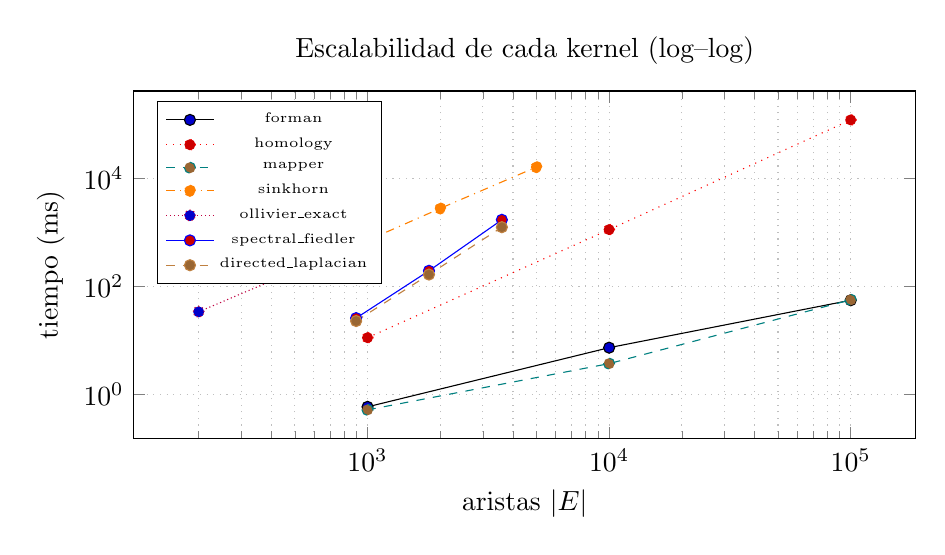
\begin{tikzpicture}
\begin{axis}[
  width=0.95\linewidth, height=6cm, xmode=log, ymode=log,
  xlabel={aristas $|E|$}, ylabel={tiempo (ms)}, title={Escalabilidad de cada kernel (log--log)},
  legend pos=north west, legend style={font=\tiny}, grid=both, grid style=dotted,
]
\addplot+[mark=*, solid, color=black] coordinates {(1000,0.58) (10000,7.28) (100000,55.32)};
\addlegendentry{forman}
\addplot+[mark=*, dotted, color=red] coordinates {(1000,11.15) (10000,1132.54) (100000,123013.55)};
\addlegendentry{homology}
\addplot+[mark=*, dashed, color=teal] coordinates {(1000,0.51) (10000,3.68) (100000,56.29)};
\addlegendentry{mapper}
\addplot+[mark=*, dashdotted, color=orange] coordinates {(1000,713.84) (2000,2802.92) (5000,16395.86)};
\addlegendentry{sinkhorn}
\addplot+[mark=*, densely dotted, color=purple] coordinates {(200,33.71) (500,193.93) (1000,719.83)};
\addlegendentry{ollivier\_exact}
\addplot+[mark=*, solid, color=blue] coordinates {(897,25.75) (1796,194.74) (3598,1721.04)};
\addlegendentry{spectral\_fiedler}
\addplot+[mark=*, dashed, color=brown] coordinates {(897,22.73) (1796,165.81) (3598,1255.42)};
\addlegendentry{directed\_laplacian}
\end{axis}
\end{tikzpicture}
\end{figure}


\subsection{Fixes de CVEs reales}
Ejecutamos la comparación vulnerable-vs-parcheado sobre commits de fix de CVEs
reales tomados de OSV / GitHub Security Advisories
(\texttt{benchmarks/run\_cves.py}; el arnés reconstruye la revisión \emph{before}
aplicando el diff inverso del commit sobre el contenido crudo, por lo que no
necesita cuota de API). Sobre 22 CVEs y 46 archivos fuente, \textbf{3 archivos
resolvieron un hallazgo}: son inyecciones \texttt{eval} ---
\texttt{senaite.core} (CVE-2026-54569; \texttt{value = eval(value)} sobre un
parámetro) y \texttt{xinference} (CVE-2026-61539; \texttt{eval(text)} sobre salida
del LLM) --- más una resolución parcial en \texttt{nltk} (CVE-2026-79676) ---
detectadas en la revisión vulnerable y limpias en el parche. Los CVEs restantes
son mayormente fixes \emph{internos a frameworks} o no-taint (SQL injection del
ORM de Django, Jinja, requests, GitPython, y argument-injection / chequeos de
integridad en NLTK): el flujo es indirecto o queda fuera de nuestro modelo de
sinks, así que el adaptador no ve nada. Esto refleja el resultado de Juliet y
localiza la frontera con precisión: MANIFOLD ya captura fixes de
\texttt{eval}/\texttt{exec}/deserialización a nivel aplicación; los flujos
mediados por frameworks necesitan análisis interprocedural, sensible al contexto
y consciente de librerías.

\subsection{Homología de caminos dirigida (GLMY)}
Implementamos la \emph{homología de caminos} $H_0,H_1$ de
Grigor'yan--Lin--Muranov--Yau sobre el 1-esqueleto dirigido
(\texttt{core/src/path\_homology.rs}): $\Omega_2^\partial$ es el conjunto de
2-caminos admisibles cuyo borde largo es admisible y no degenerado ($u\neq w$), y
los rangos se calculan por eliminación gaussiana. La dirección cambia el
veredicto. En \texttt{reentrancy.py}, la homología no-dirigida reporta
$\beta_1=1$ (el triángulo
\texttt{withdraw}/\texttt{read\_balance}/\texttt{update\_balance}), mientras que
GLMY reporta $\beta_1=0$: los 2-caminos transitivos a través del ápice
\texttt{withdraw} rellenan el 2-ciclo
\texttt{read\_balance}$\leftrightarrow$\texttt{update\_balance}. En un 2-ciclo
aislado $A\leftrightarrow B$ los papeles se invierten (GLMY $\beta_1=1$,
no-dirigida $\beta_1=0$), y el analizador devuelve el \emph{generador} de $H_1$
--- el ciclo dirigido como lista de aristas $\{A\to B,\;B\to A\}$ --- de modo que
la invariante es accionable, no solo un número. La simetrización (C2) por tanto
\emph{no} es inocua: la invariante dirigida es una señal genuinamente distinta, y
a veces opuesta.

\subsection{Ablación del LLM}
Ejecutamos el agente dos veces sobre un corpus variado de 38 archivos de Python
(29 con un hallazgo confirmado, abarcando command / code-exec / SQL /
deserialización / path-traversal / file-write / logging / SSTI, más variantes
seguras y gateadas): offline (hipotetizador heurístico) y online a través del
proxy local de \textbf{LiteLLM} (DeepSeek \texttt{flash}, compatible OpenAI
\texttt{/v1}). Los ejes de \emph{detección} y \emph{ranking} son invariantes: los
conjuntos de hallazgos confirmados y su orden por confianza coinciden en $37/38$
archivos (acuerdo $0.974$), porque el verificador SMT --- no el LLM --- es el
árbitro. La única discrepancia es un caso de \texttt{compile} (code-exec) donde
la hipótesis del LLM es en sí misma no determinista (a veces vacía), así que
ocasionalmente deja de re-proponer el hallazgo en lugar de cambiarlo. El eje de
\emph{interpretación} cambia: en $8$ de los $29$ hallazgos confirmados ($28\%$)
el LLM asigna un CWE distinto, habitualmente más específico (p.~ej.\ CWE-674
``recursión no controlada'' para el ciclo de reentrancia vs.\ la etiqueta
genérica de la heurística), y produce títulos más concisos. Esta ablación
controlada y mayor (38 archivos, \texttt{benchmarks/run\_llm\_ablation.py})
confirma la frontera de arbitraje a escala: \emph{el LLM aporta
interpretabilidad y reporte, no detección ni ranking} --- el reparto
neuro-simbólico se sostiene con una pequeña fuga de no determinismo medida. Una
ablación del lado Java/OWASP queda como trabajo futuro.

\subsection{Backend binario dual}
El adaptador binario trae dos backends intercambiables que emiten la misma IR:
(i) una ruta de texto \texttt{objdump} sin dependencias (etiquetas de función
$+$ aristas \texttt{call} $+$ alcanzabilidad de taint interprocedural) y (ii) un
backend \texttt{angr} \emph{opcional} (recuperación \texttt{CFGFast} del grafo de
llamadas interprocedural $+$ la misma alcanzabilidad de taint), seleccionable con
\texttt{--adapter angr-binary}. La ruta rápida mantiene MANIFOLD usable sin
dependencias pesadas; la ruta angr recupera flujo de control que las heurísticas
de desensamblado pierden. Esta paridad es el sustrato para futuros benchmarks
ELF/PE de SARD.

\section{Invariantes estructurales a través de dominios}
Los dos resultados hasta aquí son dos caras de una misma frontera, no dos
proyectos. De un lado (inyecciones lineales) un servlet plano y casi acíclico no
tiene curvatura ni topología persistente que explotar, y el taint clásico ya es
casi óptimo --- así que los priors estructurales no aportan. Del otro lado el
dato infractor es legítimo y solo la \emph{estructura} del programa --- sus
fronteras de privilegio y transiciones de estado --- delata el defecto, así que
la estructura es la \emph{única} señal. La misma maquinaria (grafo tipado,
álgebra de privilegios, homología dirigida, Z3) abarca ambos lados; lo que cambia
es la relación de programa que se modela. Esta sección releva los cuatro dominios
donde el análisis estático convencional es ciego y donde cada capa matemática
encuentra su lugar natural.

\subsection{Invariantes de autorización: BOLA / IDOR / BFLA}
BOLA/IDOR (CWE-639) y la autorización ausente (CWE-862) encabezan el OWASP API
Security Top~10, y el taint clásico no los ve: el selector de objeto es un valor
\emph{limpio} (un id entero, a menudo casteado), el sink es una consulta
ordinaria y el bug es que el usuario~A lee los datos del usuario~B --- no hay
dato ``sucio'' que rastrear. El objeto modelado es un grafo \emph{multipartito}:
la superficie de la API (operaciones OpenAPI), los endpoints del backend, los
decoradores de permisos (nodos \texttt{gate}) y los modelos de datos, como
produce el adaptador OpenAPI (\texttt{manifold.ingest.web}), que ya emite aristas
\texttt{auth} desde los esquemas de seguridad. La señal es el complemento de la
invariante mecanizada \texttt{no\_auth\_bounded}: un camino dirigido desde un
punto de entrada público a un recurso protegido \emph{sin} arista estricta de
autorización donde se requiere una. MANIFOLD lo implementa como el detector de
\emph{autorización ausente / BOLA}
(\texttt{manifold.analysis.authorization.bola\_idor\_candidates}), y Z3 prueba
entonces si una asignación de sesión (\texttt{session.user\_id} $\neq$
\texttt{resource.owner\_id}) alcanza el recurso --- un \emph{witness matemático
de BOLA}. En un corpus curado de 39 casos (\texttt{examples/python/bola/},
\texttt{examples/python/bola\_corpus/}, evaluado por
\texttt{benchmarks/run\_bola.py}) el taint reporta \emph{cero}
hallazgos en los casos vulnerables mientras el detector estructural alcanza
\textbf{recall $1.0$} con \textbf{precisión $0.72$} (F1 $0.837$): una señal de
factibilidad con un límite de precisión honesto, porque la heurística estructural
sobre-aproxima (los casos parametrizados/sanitizados/de fuente sin usar son los 7
falsos positivos documentados). Es precisamente el régimen donde el taint
demostrablemente puntúa $0$ y la estructura es la única señal.

\subsection{Máquinas de estado, concurrencia y protocolos: homología dirigida}
En un servlet no hay ciclos de estado; en contratos inteligentes, protocolos de
adquisición de locks y controladores de concurrencia, los peores defectos
\emph{son} ciclos de realimentación destructivos (reentrancia, deadlocks,
transiciones ilegales como \texttt{Unauthenticated} $\to$ \texttt{Authenticated}
salteando la validación de firma). El objeto modelado es el \emph{grafo de
transiciones de estado} (el CFG interprocedural extendido con llamadas externas
y mutaciones de almacenamiento global). El generador persistente dirigido de
$H_1$ de la homología de caminos GLMY es la firma exacta de un ciclo de
reentrancia --- y, como mostró \S4.2, la simetrización \emph{no} es inocua: la
homología no dirigida puede reportar $\beta_1=1$ donde GLMY reporta $0$ (un
triángulo rellenado por un ápice) y viceversa. Sobre un ciclo de adquisición de
locks sintético (\texttt{examples/state\_machine/lock\_cycle.json}) el análisis
dirigido extrae el generador concreto $[\,s_0\!\to\!s_1,\ s_1\!\to\!s_2,\
s_2\!\to\!s_0\,]$ con $\beta_1=1$ --- un hallazgo sin análogo en taint.

\subsection{Topologías de confianza, IAM y movimiento lateral}
En entornos cloud (AWS/Azure/Kubernetes) las peores brechas vienen de
\emph{cadenas} de escalada de privilegios y movimiento lateral (un rol
comprometido en un frontend asumiendo un rol secundario con acceso a un bucket de
secretos). El objeto modelado es el \emph{grafo de identidades y permisos}
(usuarios, roles IAM, políticas de confianza, servicios, recursos de red). Aquí
el corte de Fiedler ($\lambda_2, f_2$) particiona óptimamente los dominios de
confianza (p.~ej.\ DMZ vs.\ núcleo); las aristas que cruzan el corte sin
controles intermedios emergen como anomalías espectrales en la frontera de
confianza, y la curvatura de Forman--Ricci --- lejos de ser un error de
detección --- \emph{aisla los puentes de privilegio críticos}: un nodo con
$\kappa_F$ fuertemente negativa es un rol o credencial que es el único puente
entre dos subredes de confianza dispares (el pivote ideal del atacante). El
agente entrega entonces los caminos sugeridos a Z3, que resuelve la combinatoria
de políticas IAM para confirmar si la cadena de asunción de roles es viable.

\subsection{Seguridad de agentes autónomos y LLMs}
Los sistemas modernos que conectan LLMs a herramientas externas (APIs, bases de
datos, shell, correo) enfrentan ataques de \emph{confused deputy} e inyección
indirecta de prompt. El objeto modelado es el \emph{grafo de uso de
herramientas}: usuario, modelo, memoria contextual y herramientas externas a
distintos niveles de privilegio, con aristas tipadas \texttt{untrusted\_input}
(datos web, correo leído) y \texttt{privileged\_execution} (borrar una base de
datos, emitir pagos, ejecutar comandos). El defecto es una violación de la
invariante de autorización: un flujo de entrada no confiable que alcanza una
herramienta de ejecución privilegiada sin un \texttt{gate} explícito de
sanitización o confirmación humana. Esto es exactamente lo que el adaptador
\texttt{llm-agent} (\texttt{manifold.ingest.llm\_agent}) ya detecta: una
herramienta peligrosa alcanzable desde la entrada del usuario sin una puerta de
aprobación es un hallazgo.

\subsection{Matriz de mapeo y posicionamiento}
\begin{center}
\small
\begin{tabular}{@{}p{0.26\linewidth}p{0.36\linewidth}p{0.32\linewidth}@{}}
\toprule
\textbf{Capa formal / matemática} & \textbf{Objeto modelado} & \textbf{Vulnerabilidad mapeada} \\
\midrule
Invariante auth (Lean 4) & endpoints, decoradores, recursos de API & BOLA / IDOR / BFLA \\
Homología dirigida (GLMY) & grafo de transiciones de estado y llamadas asíncronas & reentrancia, desincronización de estado, deadlocks \\
Espectral (Fiedler) & topologías de red, Kubernetes RBAC, IAM & ruptura de segmentación de confianza, movimiento lateral \\
Curvatura discreta (Ricci) & grafos de microservicios e identidad & puntos únicos de fallo, puentes de escalada de privilegios \\
Verificador simbólico (Z3) & restricciones de camino en la lógica de negocio & contraejemplos ejecutables (witnesses) \\
\bottomrule
\end{tabular}
\end{center}
MANIFOLD se reposiciona así como un \emph{motor formal de invariantes
estructurales y lógica de negocio}, no como competidor de Semgrep/CodeQL en
patrones locales de SQLi/XSS. (1) \emph{Abandona una competencia estéril}: no
intenta ganarle al taint en un servlet de 20 líneas. (2) \emph{Ataca lo que nadie
resuelve}: fallas de diseño, coherencia de privilegios, protocolos concurrentes y
arquitecturas de agentes, donde las reglas sintácticas callan porque el código,
línea por línea, parece legítimo. (3) \emph{Mantiene intacto el software}: la IR
tipada, los núcleos en Rust, la verificación en Lean~4, el orquestador Z3 y el
agente neuro-simbólico se preservan íntegramente, aplicados sobre el grafo de
relaciones adecuado. La narrativa no es, por tanto, ``la geometría perdió contra
el taint'' sino una única cuenta de \emph{qué} relaciones de programa hacen
informativas a las invariantes estructurales: una frontera negativa rigurosamente
establecida en SAST de inyección lineal, y una positiva en los defectos
arquitectónicos donde el taint es ciego --- ambos lados respaldados por código
funcional y datos medidos.

\begin{thebibliography}{9}
\item M.~Fiedler, \emph{Algebraic connectivity of graphs}, 1973.
\item F.~Chung, \emph{Spectral Graph Theory}, 1997.
\item Edelsbrunner, Letscher, Zomorodian, \emph{Topological persistence and simplification}, 2002.
\item Singh, M\'emoli, Carlsson, \emph{Topological Methods for the Analysis of High Dimensional Data Sets}, 2007.
\item Y.~Ollivier, \emph{Ricci curvature of Markov chains on metric spaces}, 2009.
\item P.~Cousot \& R.~Cousot, \emph{Abstract interpretation: a unified lattice model}, 1977.
\item S.~Mac~Lane, \emph{Categories for the Working Mathematician}, 1971.
\item J.~King, \emph{Symbolic execution and program testing}, 1976.
\item E.~M.~Clarke et al., \emph{Automatic verification of finite-state concurrent systems}, 1986.
\item F.~Chung, \emph{Laplacians and the Cheeger inequality for directed graphs}, 2005.
\item Grigor'yan, Lin, Muranov, Yau, \emph{Homotopy theory for digraphs}, 2012.
\item M.~Cuturi, \emph{Sinkhorn distances: lightspeed computation of optimal transport}, 2013.
\item R.~Forman, \emph{Bochner's method for cell complexes and combinatorial Ricci curvature}, 2003.
\item L.~de~Moura \& N.~Bj\o rner, \emph{Z3: An efficient SMT solver}, 2008.
\item Y.~Shoshitaishvili et al., \emph{SoK ... (angr)}, 2016.
\item OWASP Foundation, \emph{OWASP Benchmark v1.2}, 2016--2024.
\item OWASP Foundation, \emph{OWASP API Security Top 10} (API1:2023 Broken Object Level Authorization), 2023.
\item NIST, \emph{SARD / Juliet Test Suite}, 2017.
\item BerriAI, \emph{LiteLLM}, 2023--2024.
\item SonarSource, \emph{SonarQube} (Community Edition, reglas SonarJava).
\item GitHub, \emph{CodeQL} y la suite \texttt{java-security-extended}.
\end{thebibliography}

\end{document}
